%------------------------------------------------------------------------------
% This is a LaTeX template for the scientific justification of IRAM Proposals 
%------------------------------------------------------------------------------
% 
% We encourage IRAM proposers to use this template for the sake of unity 
% and clarity when Program Committee members assess their proposals.
% 
% You may customize this template to suit your preferences (e.g. using BibTex),
% but please respect the following requirements:
%     The scientific justification should contain a maximum of 2 pages of text 
%     (4 pages for Large Programs), plus 2 pages of Figs., Tables and Refs.
%     The font size should be 11pt or larger.
%
% For Large Programs, the following sections should be included: 
%   i) Scientific Rationale, 
%  ii) Immediate Objective, 
% iii) Feasibility and Technical Justification, and 
%  iv) Organizational Issues.
% 
%
%------------------------------------------------------------------------------
%
\documentclass[11pt,a4paper,twoside,graphicx,color]{article}
%
\usepackage[margin=2cm]{geometry}
\usepackage[pdftex]{graphicx}
\usepackage{color}
\usepackage{txfonts}
\usepackage{paralist}
\usepackage[numbers]{natbib}
\setlength{\bibsep}{0.0pt}
\usepackage{amssymb}

\newcommand{\ccor}[1]{\textcolor{red}{#1}}

%
% Page size and text dimensions
% Do not change!
\textheight 260mm
\textwidth 178mm
\oddsidemargin -8mm
\evensidemargin -8mm
\marginparwidth 50pt
\topmargin -22mm
\brokenpenalty=10000
\sloppy
%
%-------------------------------------------------------------------
\begin{document}
\def\moo{MOO\,J1142$+$1527}
%
%
\begin{center}{\huge \bf
%-------------------------------------------------------------------
High resolution SZ observations of the massive and distant cluster \moo\ with NIKA2
%-------------------------------------------------------------------
}\end{center}
% 
\centerline{\bf P.I.: F. Ruppin \& B. Comis}

\section{Scientific context}
Galaxy clusters are the ultimate manifestation of the hierarchical structure formation process, and as such, they are sensitive to both the matter content and expansion history of the Universe. %Clusters of galaxies are thus powerful tools to characterize the \textbf{formation processes of large scale structures}. Although hierarchical gravitational collapse of small structures seems to be the main driver of cluster formation, non-gravitational processes such as feedback from AGN and supernova-driven galactic winds may alter cluster observables to a large extent. Consequently a detailed characterization of the complex interplay between gravitational and non-gravitational processes acting on clusters is mandatory for \textbf{a detailed understanding of their astrophysics}.
\textbf{In particular, the high mass tail} of the galaxy cluster population is of significant interest for cosmology as well as for large scale structure formation and galaxy evolution. For cosmology, massive, high-redshift clusters can provide an extremely powerful complementary probe to constrain the accelerated expansion of the Universe and its content in different ways (e.g. the evolution of the cluster mass function \cite{vik09}).%, the clustering of galaxy clusters \cite{ser15}, and through application of the $f_{gaz}$ test \cite{man14}. The high mass tail of the galaxy cluster mass function is also a sensitive indicator of primordial non-Gaussianity \cite{sha13}.

The principal baryonic component of galaxy clusters is found in the hot, ionized, X-ray emitting gas of the intracluster medium (ICM), containing about 12\% of the total mass. This gas produces a key cluster observable, \textbf{the thermal Sunyaev-Zel'dovich effect} (tSZ) \cite{sun72} which is due to the inverse Compton scattering of cosmic microwave background (CMB) photons with high energy electrons of the ICM. As the amplitude of this effect (the Comptonization parameter, $y$) is directly proportional to the thermal energy contained in the ICM ($y~\propto~\int P_e dl$), it is expected to provide a low scatter mass proxy for galaxy clusters \cite{nag07}. Furthermore, as the tSZ effect is a CMB spectral distortion, it does not suffer from cosmological dimming and its peculiar spectral behavior (CMB flux decrement/increment at frequencies respectively below/above 217~GHz) makes it an efficient cluster identifier. This observable is therefore a powerful probe to detect clusters and characterize their baryonic content distribution \textbf{up to very high redshift}.
In the last years, the SZ dedicated instruments SPT, ACT and Planck have been used to conduct wide-area surveys at millimeter wavelengths and identify galaxy clusters via the SZ effect, with several tens of massive clusters at $\mathbf{z > 1}$. However, beside the powerful role of SZ in detecting high-$z$ objects, the upcoming generation of infrared-selected galaxy-based cluster searches can also complement the work of past and future millimeter surveys, exploring large volumes to detect the rarest high-mass and high-$z$ clusters in our Universe. 

\textbf{The Massive and Distant Clusters of WISE Survey} (MaDCoWS) has been designed to detect the most massive galaxy clusters at $z \sim$ 1. It offers the largest survey area among current high-redshift cluster searches, using infrared WISE and PanSTARRS optical imaging to robustly isolate galaxy clusters at $z \sim 1$ over more than 80\% of the extragalactic sky. The SZ decrements of several MaDCoWS detections have been obtained with CARMA (Combined Array for Research in Millimeter-wave Astronomy, \cite{brodwin15}, \cite{gonz15}), showing that their selection leads to the discovery of evolved, hot, massive galaxy clusters that represent excellent candidates for detailed SZ follow-ups. The results obtained have demonstrated that MaDCoWS is able to find the SPT-like massive and high-$z$ clusters outside of the SPT footprint, north of $\delta > -30\deg$..

MaDCoWs and Planck cover a significant fraction of the extragalactic sky, but Planck SZ blind detections concentrate on massive objects at $z~<~$0.8. However, in the near future, we plan to cross-correlate the MaDCoWS targets with the Planck SZ full sky map ($y$-map), to select a sample of robust candidates for future NIKA2 follow-ups. With a selection function independent of the ICM properties, the MaDCoWs sample will be closer to the future Euclid and LSST cluster catalogues. The Planck+NIKA2 SZ view of such objects will thus contribute to a more complete description of galaxy cluster gas content distribution also for richness (i.e. number of galaxies) selected catalogues of clusters. These upcoming optical/IR surveys will have the combination of sensitivity and area to push cluster detection to the $z \geq 2$ regime.
%In the coming years such IR/optical surveys will provide interesting cluster samples for the high-mass and high-redshift population. And these will of course represent further interesting targets for the NIKA2 camera and SZ science. MaDCoWS will permit an unbiased z ? 1 calibration of these scaling rela- tions using clusters selected independently of the strength of the intracluster medium.
%Combining the sub-arcminute resolution NIKA2 SZ data with the Planck view of such clusters, we will also explore the possible impact and future perspectives of combining the complementarity of these two SZ instruments to contribute to the characterization of the high-z high-mass cluster populations, in terms of mass-observable calibration and understanding of .

\noindent {\bf \large Proposed observations -- }
We propose to observe the massive galaxy cluster \moo\ at $z = 1.19$, which was originally identified by the MaDCoWS project. We intend to observe it as a first high angular resolution SZ observation with NIKA2 for such a high redshift infrared detected massive object. The existence of \moo\ is not in tension with the $\Lambda$CDM paradigm, but such clusters are expected to be extremely rare. Indeed, there are predicted (for Planck cosmology) to be only $\sim 7$ such massive clusters of galaxies over the full sky at $z >1.19$ in the standard cosmological model (see Fig. \ref{fig:SZ_MOO} right panel). 
%Within the WMAP9 and Planck cosmologies, there are predicted to only be $\sim 3$ or $\sim 7$ clusters this massive over the full sky at $z >1.19$, respectively, and only $\sim 1-2$ within the corresponding SDSS survey area (see Fig. \ref{fig:SNRprof} middle panel). 
A full characterization of this cluster ICM would therefore bring insights on the entanglement between very high redshift cluster morphology and dynamical properties.

\noindent {\bf \large Previous observations with NIKA -- } 
The NIKA prototype has been used as a pathfinder for NIKA2, to demonstrate the possibility to use large arrays of Kinetic Inductance Detectors (KIDs) in millimeter astronomy and to validate the observation strategy as well as the data analysis. It has already proven to be particularly adapted for tSZ observations at intermediate and high redshifts. Five papers have been published based on the 6 galaxy cluster SZ observations with NIKA at the IRAM 30~m telescope. NIKA has validated its capabilities to probe the details of ICM physics at intermediate ($z=0.45$ for RX~J1347.5-1145 \cite{ada14}) and high redshift ($z=0.89$ for CL~J1226.9+3332 \cite{ada15}), to deal with point sources contamination (MACS~J1423.8+2404 \cite{ada16a}), to reach the sensitivity required to produce the first significant kinematic SZ effect mapping (MACS~J0717.5+3745 \cite{ada16b}). Eventually, the follow-up of the Planck discovered cluster PSZ1~G045.85+57.71 allowed us to make the first non-parametric deprojection of a combination of large field-of-view (Planck) and high angular resolution (NIKA) SZ observations at intermediate redshift \cite{rup16}. NIKA2 at the IRAM 30~m telescope is perfectly adapted to probe the inner structure of galaxy clusters and to undertake a high angular resolution follow-up of optically detected very massive and very distant cluster.

%-------------------------------------------------------------------
\section{Technical justification}
{\bf \large Target selection -- }
We intend to observe \moo\ as a first SZ study of the high mass and very high redshift cluster population with NIKA2. This cluster has been selected according to the following criteria: \textbf{(1)} - IR/Optically discovered cluster. \textbf{(2)} - Very high redshift (z~=~1.19) and very massive cluster ($M_{500} = (6.0 \pm 0.9) \times 10^{14} M_{\odot}$, $M_{200m} = (1.1 \pm 0.2) \times 10^{15} M_{\odot}$): one of the rarest objects in the sky (Fig. \ref{fig:SZ_MOO} right panel). \textbf{(3)} - SZ confirmed detection, as it has been observed also with CARMA for approximately 5 hours on-source (Fig. \ref{fig:SZ_MOO}, left panel) and we have a significant positive signal at the cluster position on the Planck Comptonization parameter map (Fig. \ref{fig:SZ_MOO}, middle panel). \textbf{(4)} - Good visibility during the observation period (elevation $>~50^\circ$ for 5 hours everyday in January 2017 see Fig. \ref{fig:technical} left panel). \textbf{(5)} - Interesting morphology (the CARMA map of this cluster displays an elliptical ICM morphology which may indicate the presence of unrelaxed structures). 
In synthesis, \textbf{\moo\ represents an extremely interesting target, while also being adapted to a first shared-risk open pool of the new instrument NIKA2.} We know several properties of this object, which has been detected and studied at different wavelengths. It has already been observed in SZ and its flux is expected to be very strong. A brief description of \moo\ is given in Tab. \ref{tab:moo_reference}. {\color{red}This cluster is in the Chandra queue (PI Stanford).  There is deep HST data in F105W and F140W (along with shallow F814W).  We also have fairly deep Gemini r' and z' band data, as well as very deep GTC GRI data.  A 48 ks Chanda ACIS-I exposure is forthcoming.}

\noindent {\bf \large Immediate outputs -- }
Our project aims at detecting and characterizing the tSZ signal in 1D (profile) and 2D (map) up to $\sim 6'$. We intend to: \textbf{(1)} – Map the tSZ signal of this cluster in order to constrain its morphology at high angular resolution. \textbf{(2)} – Extract the thermal pressure distribution using a non-parametric deprojection of the tSZ observation (\cite{rup16}). This will be compared to the universal pressure profile constrained on a sample of low redshift clusters ($z < 0.3$ see \cite{arn10}). \textbf{(3)} – Derive the global tSZ signal $Y_{SZ}$ and compare it to the measurement made by the CARMA collaboration. \textbf{(4)} – Compare the thermodynamical and dynamical properties of this cluster with outputs from numerical simulations such as MUSIC \cite{sem14} to constrain the cluster formation history.
{\color{red}This cluster is in the Chandra queue (PI Stanford).  We should probably mention this, and point out that this proposal will allow a direct comparison of the SZ and X-ray views of high-resolution ICM structures in a $z >$ 1 cluster.}

\noindent {\bf \large Scanning strategy and time estimate requirements -- }
We used the time estimator provided by IRAM to estimate the observing time. The sensitivity of the NIKA2 camera is expected to be 20 mJy.s$^{1/2}$ at 150 GHz and 30 mJy.s$^{1/2}$ at 260 GHz.\\
We will use on the fly scans of 10'$\times$8' with different orientations along the azimuth and elevation directions. This will allow us to properly define the zero level of our map and measure angular scales structures up to 6'. About one half of the observing time will be spent on the core of the signal. \\
In the case of tSZ observations, we assume calibration overheads (focus, pointing, photometry) to account for not more than 25\% of the overall observing time, as it was the case for the NIKA winter pool of February 2014. Nevertheless we kept the original overhead of 50\% and considered 2~mm of water vapor in the atmosphere when using the IRAM time estimator to have a \textbf{robust time estimation} for this shared risk open time observation.\\
Taking into account uncertainties on the tSZ flux estimates, and in order to reach a {\bf SNR of more than 9} at the clusters peak ({\it i.e.} a RMS of 0.33 mJy/beam on the map), we need 7.5 hours of on-target observations. Including calibration (focus, pointing, photometry), we therefore request 15 hours of observations to reach the scientific objectives for this cluster. Such observing time will allow us to get a \textbf{signal-to-noise ratio higher than 3 on the SZ surface brightness profile at $\mathbf{\theta_{500}}$} (see Fig. \ref{fig:technical} right panel) and therefore to characterize precisely the pressure distribution within the ICM.

\noindent {\bf \large Data processing -- }
Our team has reached a deep expertise, developing an SZ pipeline for NIKA and NIKA2 data (5 papers published since 2013). The two PIs are part of the NIKA2 Collaboration and Core Team and they are also significantly involved in the commissioning of the NIKA2 camera, to achieve a complete optimization and characterization of the instrument.

%-------------------------------------------------------------------

\begin{table}[h]
\begin{center}
\resizebox{\textwidth}{!} {
\begin{tabular}{|p{3.1cm}|p{1.6cm}|p{1.6cm}|p{0.6cm}|p{2.6cm}|p{6.8cm}|}
\hline
Cluster & R.A. & Dec. & $z$ & $Y_{500}$ (Mpc$^2$) & Comment \\
\hline
\hline
\moo\ & 11:42:46.6 & $+15$:27:15 & 1.19 & $(9.7\pm 1.3) \times 10^{-5}$&  {\footnotesize Observed with WISE, Spitzer and CARMA. tSZ peak at about 10~mJy/beam. Hosts a NVSS radio point source (NVSS J114247+152711, 3.4 mJy at 31 GHz measured with CARMA.)}\\
\hline
\end{tabular}
}
\end{center}
\caption{\footnotesize Brief characteristics of the proposed cluster.}
\label{tab:moo_reference}
\end{table}

\begin{figure}[h]
\centering	
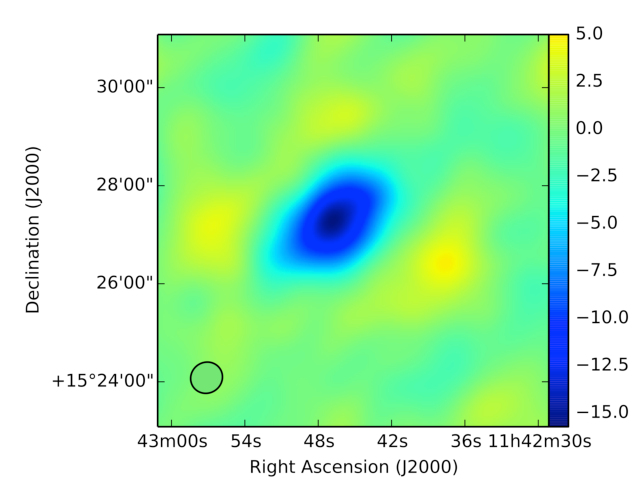
\includegraphics[width=0.34\textwidth]{./cluster.pdf}   
\hspace{0.13cm}
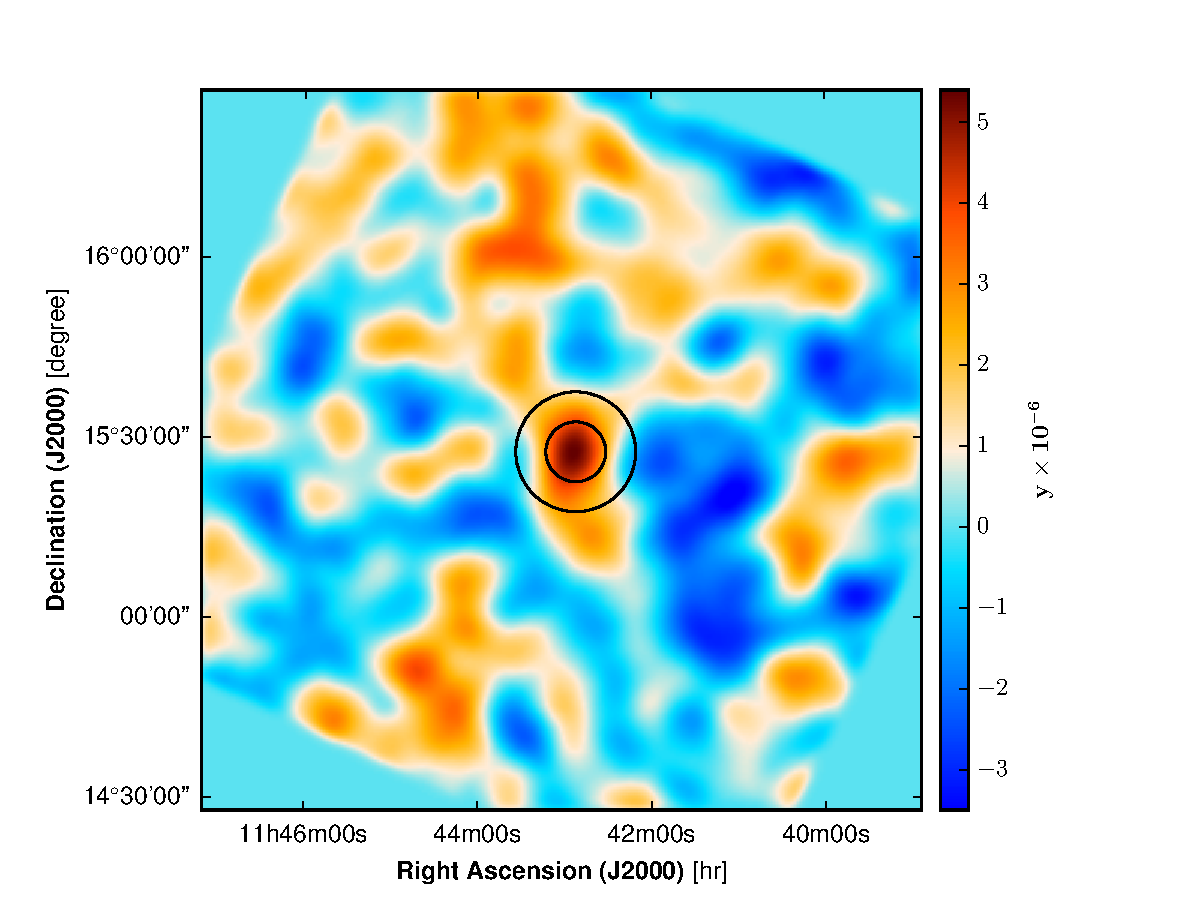
\includegraphics[width=0.35\textwidth]{.//MOO_Planck_3.pdf}
\hspace{-0.5cm}  
 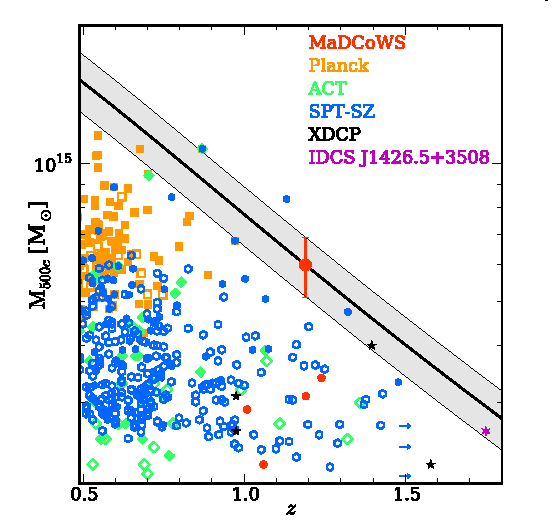
\includegraphics[width=0.3\textwidth]{./redshift_mass.pdf}   
\caption{\footnotesize Left: CARMA SZ map of \moo\ covering a $8' \times 8'$ field in signal-to-noise unit. Middle: Planck Comptonization parameter map centered at the nominal position of \moo\  (the black circles have radii of respectively 5' and 10'). Right: Comparison in the mass-redshift plane of \moo\ (large red circle with error bars) with other MaDCoWS clusters (red circles) and clusters from other surveys.}
\label{fig:SZ_MOO}
\end{figure}

\begin{figure}[h!]
\centering	
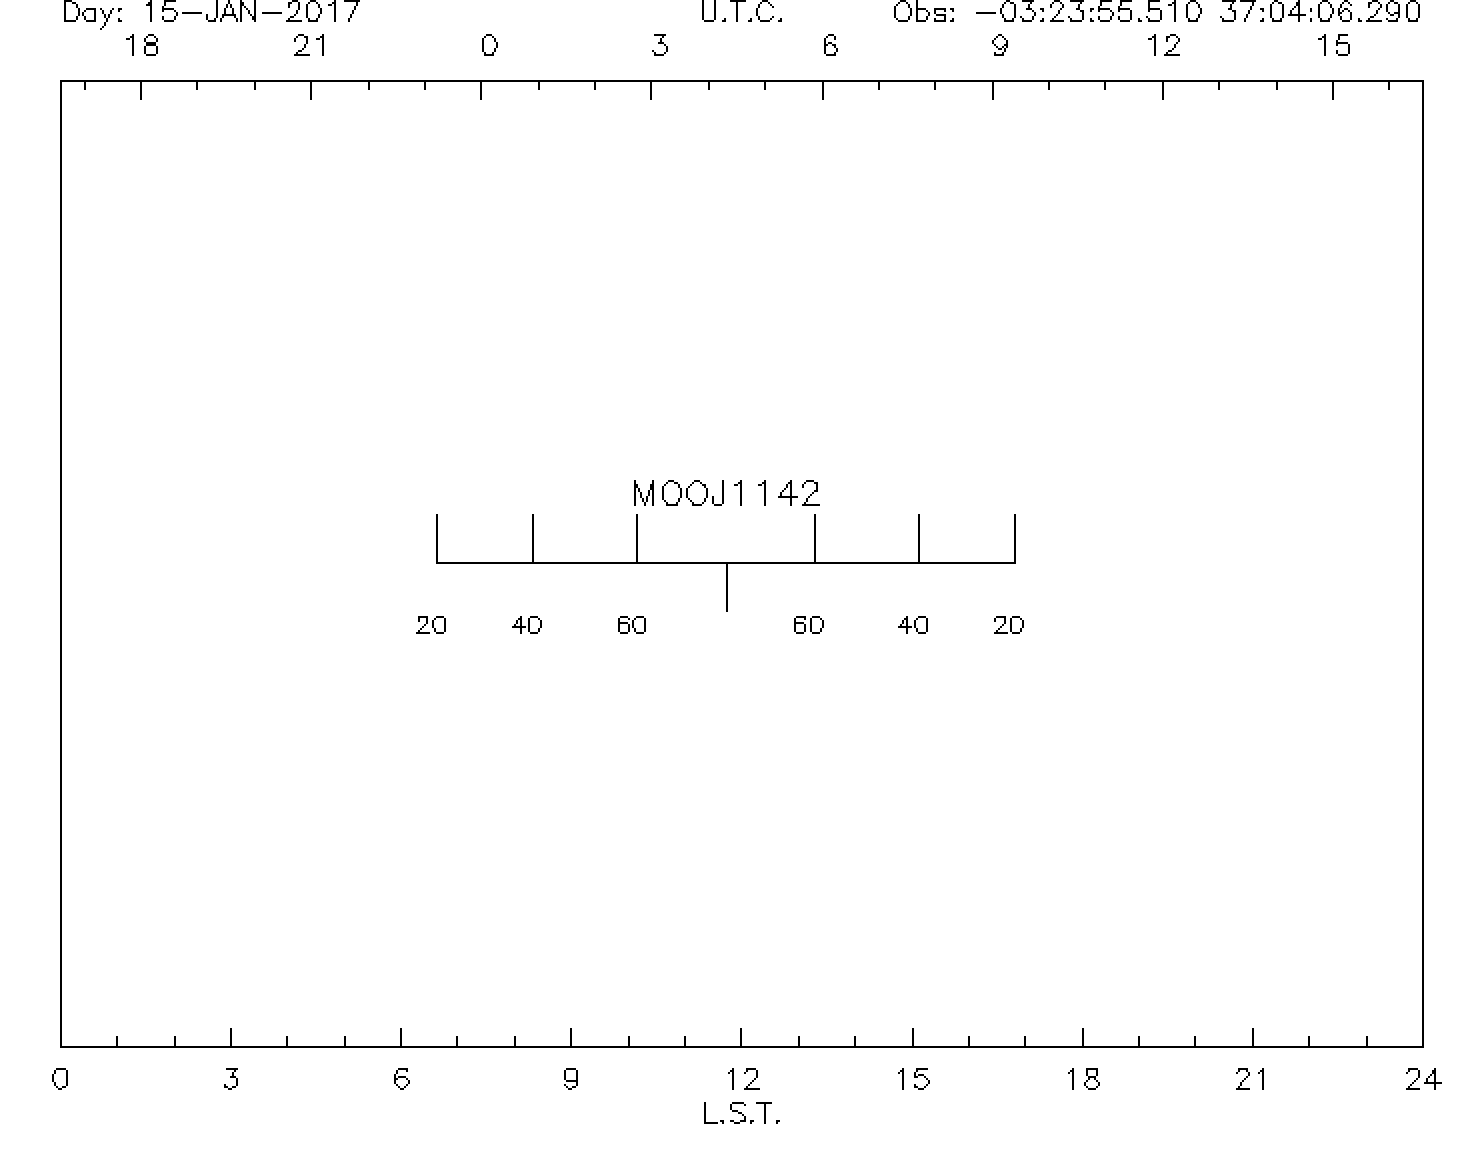
\includegraphics[width=0.35\textwidth]{./sky_trajectory.png}
\hspace{1.5cm}
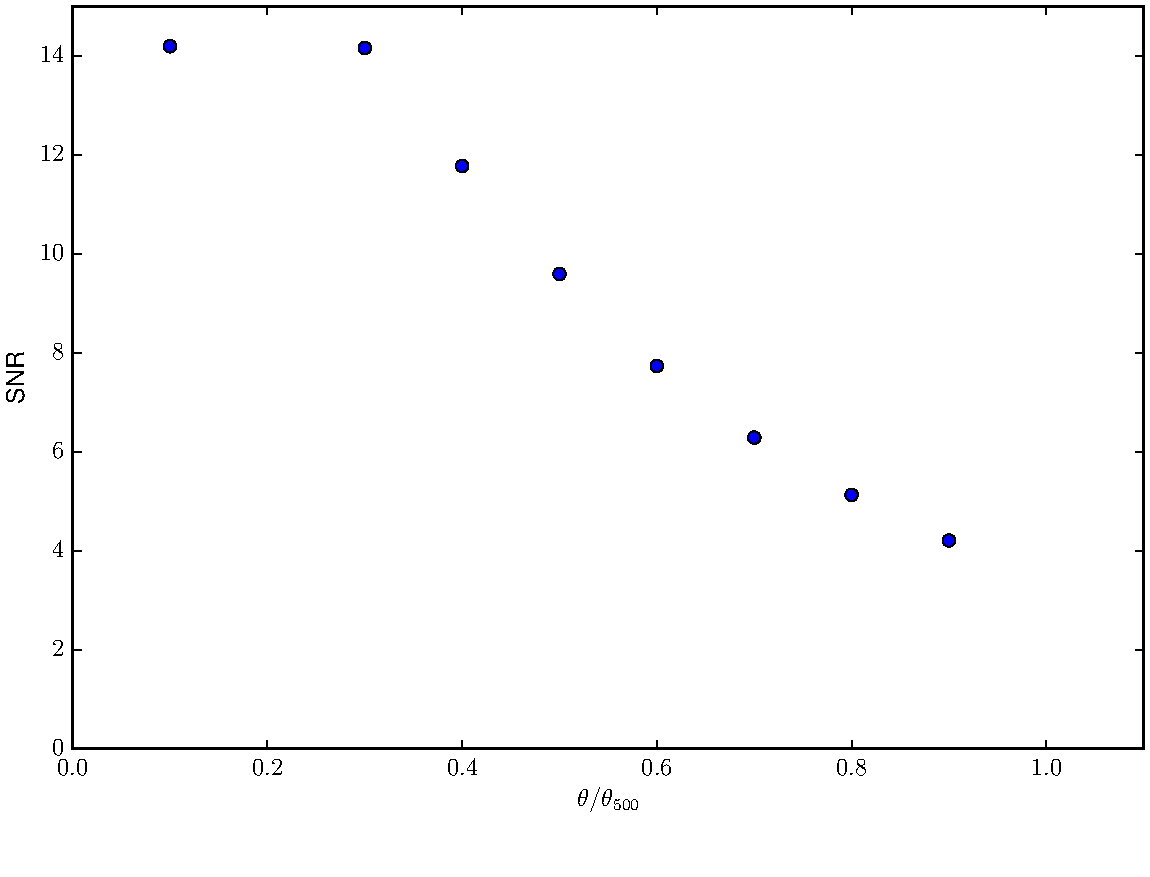
\includegraphics[width=0.33\textwidth]{./MOOJ1142_snr_prof.pdf}  
\caption{\footnotesize Left: \moo\ presence in the sky at the IRAM 30~m telescope in January 2017. Right: Expected signal-to-noise profile for a total observing time of 15 hours with NIKA2.}
\label{fig:technical}
\end{figure}

\begin{thebibliography}{9}

\bibitem[Sif{\'o}n et al.(2016)]{sif16}
 {\small C. Sif{\'o}n, N. Battaglia,  M. Hasselfield, {\it et al.} (2016) MNRAS, \textbf{461}, 248-270}

\bibitem[Pratt et al.(2009)]{pra09}
 {\small G.~W. Pratt, J.~H. Croston,  M. Arnaud, {\it et al.} (2009) A\&A, \textbf{498}, 361-378}

\bibitem[Hoekstra et al.(2015)]{hoe15}
 {\small H. Hoekstra, R. Herbonnet,  A. Muzzin, {\it et al.} (2015) MNRAS, \textbf{449}, 685-714}

\bibitem[Sunyaev \& Zeldovich(1972)]{sun72}
  {\small R. A. Sunyaev, \& Y. B. Zel'dovich (1972), Astrophys. Space Phys. Res., \textbf{4}, 173}
  
  \bibitem[Nagai et al.(2007)]{nag07}
  {\small D. Nagai, A.~V. Kravtsov, A. Vikhlinin, {\it et al.} (2007), ApJ, \textbf{668}, 1-14}
  
  \bibitem[Brodwin et al.(2015)]{brodwin15}
   {\small M. Brodwin, C. H. Greer, E. M. Leitch, {\it et al.} (2015), ApJ, \textbf{806}, 26}

  \bibitem[Gonzalez et al.(2015)]{gonz15}
  {\small A. H. Gonzalez, B. Decker, M. Brodwin, {\it et al.} (2015), ApJL, \textbf{812}, L40}
  
  \bibitem[Mantz et al.(2014)]{man14}
   {\small A.~B. Mantz, S.~W. Allen, R.~G. Morris, {\it et al.} (2014), MNRAS, \textbf{440}, 2077}
  
  \bibitem[Vikhlinin et al.(2009)]{vik09}
   {\small A. Vikhlinin, A.~V. Kravtsov, R.~A. Burenin (2009), ApJ, \textbf{692}, 1060}
  
  \bibitem[Sereno et al.(2015)]{ser15}
   {\small M. Sereno, A. Veropalumbo, F. Marulli, {\it et al.} (2015), MNRAS, \textbf{449}, 4147}
  
  \bibitem[Shandera et al.(2013)]{sha13}
   {\small S. Shandera, A.~B. Mantz, B. Rapetti, {\it et al.} (2013), Cosmology~Astropart.~Phys., \textbf{8}, 4}
  
  \bibitem[Adam et al.(2014)]{ada14}
   {\small R. Adam, B. Comis, J.-F. Mac\'ias-P\'erez, {\it et al.} (2014) A\&A, \textbf{569}, A66}

  \bibitem[Adam et al.(2015)]{ada15}
   {\small R. Adam, B. Comis, J.-F. Mac\'ias-P\'erez, {\it et al.} (2015) A\&A, \textbf{576}, A12}

  \bibitem[Adam et al.(2016)]{ada16a}
   {\small R. Adam, B. Comis, I. Bartalucci, {\it et al.} (2016) A\&A, \textbf{586}, A122}

  \bibitem[Adam et al.(2016)]{ada16b}
   {\small R. Adam, I. Bartalucci, G.W. Pratt, {\it et al.} (2016) arXiv:1606.07721}

  \bibitem[Ruppin et al.(2016)]{rup16}
  {\small F. Ruppin, R. Adam, B. Comis, {\it et al.} (2016) arXiv:1607.07679}

  \bibitem[Arnaud et al.(2010)]{arn10}
   {\small M. Arnaud, G.~W. Pratt, R. Piffaretti, {\it et al.} (2010) A\&A, \textbf{517}, A92}

  \bibitem[Sembolini et al.(2014)]{sem14}
   {\small F. Sembolini, M. De Petris, G. Yepes, {\it et al.} (2014), MNRAS, \textbf{440}, 3520}
  
\end{thebibliography}

\end{document}
